%%%%%%%%%%%%%%%%%%%%%%%
%%%%%%%% EPL %%%%%%%%%%
%%%%%%%%%%%%%%%%%%%%%%%

\documentclass[doublecol,final,edchoice]{epl2}

\usepackage{amsmath}
\usepackage{amssymb}

\makeatletter
\setlength\arraycolsep{2pt}
\makeatother

\vol{110}
\issue{1}
\year{2015}
\firstpage{1}
\doi{10.1209/0295-5075/110/20002}
\pgid{20002}
\received{10 January 2015}
\acceptedinfinalform{7 April 2015}
\paperpub{April 2015}
\onlinepub{29 April 2015}

\title{Network topology with broken Onsager symmetry allows\\
directional and highly efficient energy transfer\vspace*{-6.3pt}}

\shorttitle{Network topology Onsager symmetry and energy transfer}

\author{B. Sabass}

\shortauthor{B. Sabass}

\institute{Mechanical and Aerospace Engineering, Princeton University - Princeton, NJ, USA}

\pacs{05.70.Ln}{Nonequilibrium and irreversible thermodynamics}
\pacs{05.60.Cd}{Classical transport}
\pacs{05.45.Xt}{Synchronization; coupled oscillators}

\abstract{~Time-reversal symmetry of most conservative forces constrains the properties of linear transport in physical systems. Here, we study the efficiency of energy transfer in dissipative oscillator networks where time-reversal symmetry is broken locally by Lorentz-force--like couplings. Despite their linearity, such networks can exhibit mono-directional transport and allow isolation of energy transfer in subsystems. New mechanisms and general rules for mono-directional transport are discussed. Combining network topology with Lorentz-force--like coupling, we show how efficiency at maximum power can surpass the common bound of 1/2 and may even approach unity.}

\begin{document}

\maketitle

\section{Introduction}

Onsager symmetry holds for the vast majority of coupled linear phenomena on the mesoscopic and macroscopic scale. However, the symmetry of transport coefficients is generally lost when time-reversal symmetry is broken through a magnetic field. Recently, it has been suggested that magnetic breaking of Onsager symmetry may allow for the existence of finite-time heat engines with vanishing entropy production and also allow an efficiency at maximum power that exceeds the Curzon-Ahlborn limit~\cite{epl17030bib1}. Although subsequent studies established a number of positive lower bounds for entropy production in concrete quantum-mechanical systems~\cite{epl17030bib2,epl17030bib3,epl17030bib4, epl17030bib5}, and classical heat engines~\cite{epl17030bib6, epl17030bib7}, the results highlight the non-trivial nature of coupled transport in the presence of a magnetic field. A logical next step is to combine the properties of magnetic couplings with topological features of a network.

Networks with classical oscillators, such as vibrating spring-damper collections, electric power grids~\cite{epl17030bib8, epl17030bib9}, or electronic circuits are omnipresent in daily life. Desired system properties, \textit{e.g.}, in terms of frequency response or current rectification, often require active or non-linear elements, such as amplifiers or diodes. We hypothesize here that linear elements that break Onsager symmetry could be a possible alternative. Such elements can be built in a variety of ways: mechanically, a coupling via Lorentz forces can be realized with a charge on a forced, two-dimensional pendulum in a magnetic field. Alternatively, electrical circuits can be connected via perpendicular sides~of~a~Hall element, which is called a gyrator~\cite{epl17030bib10,epl17030bib11, epl17030bib12}. Also, similar devices with microwaves are based on the Faraday effect~\cite{epl17030bib13}.~In principle, even Coriolis forces can be employed as a time-reversal symmetry-breaking\break coupling.

In this letter, systems of linear oscillator equations are studied as a generic model for the above examples. \nobreak{Oscillators} interact by time-reversal symmetric forces as well as through Lorentz-force--like couplings.~In spite of the simplicity, these systems are found to exhibit a rich linear response and unusual energetics.~Two aspects are \nobreak{particularly} notable.~Namely the possibility of fixing a transport direction through network properties and a highly efficient energy transfer.~While details of the system matter for mono-directional transport, network topology imposes very general and easily perceivable constraints. Corresponding rules are provided. Next, general limits for the efficiency are assessed. It is shown that both network loops and breaking of Onsager symmetry are necessary to remove technically important constraints on linear energy transfer. Finally, the system behavior in the presence of additive and multiplicative noise is discussed briefly.

\section{Framework}

Our networks consist of coupled real variables $x_j(t)$ that obey a Langevin equation as
\begin{equation}%eq1
\ddot{x}_j = -\sum_l\left(\kappa_{jl}\,x_l + b_{jl}\,\dot{x}_l\right)-\gamma_j\,\dot{x}_j + \xi_j + f_j.
\label{epl17030eqn1}
\end{equation}
The symmetric matrix $\bm{\kappa}=\bm{\kappa}^{T}$ represents, \textit{e.g.}, elastic constants for a mechanical system or capacitance for an electric network. $\bm{\kappa}$ must be positive definite for \nobreak{stability}~\cite{epl17030bib14}. The antisymmetric matrix $\mathbf{b} = -\mathbf{b}^{T}$ represents Lorenz-force--like couplings. $\gamma_j$ are positive friction constants. The noise $\xi_j$ obeys $\langle\xi_j(t)\rangle = 0$ and $\langle \xi_j(t) \xi_l(t')\rangle = \delta_{jl} 2 \gamma_j k_{\text{B}}T \delta(t-t')$ with the thermal energy $k_{\text{B}}T$. We \nobreak{assume} that the two of the oscillators with indices $a$ and $b$ are driven as
\begin{equation}%eq2
f_{\{a,b\}} = 2\,F_{\{a,b\}} \cos(\omega t + \varphi_{\{a,b\}}), \quad f_{j\,\notin \{a,b\}} = 0,
\label{epl17030eqn2}
\end{equation}
where $\omega$ is a fixed angular frequency. Phase differences will be written as $\varphi_{jl}\equiv\varphi_{j}-\varphi_{l}$. Non-dimensional units\footnote{We fix a force scale $\hat{F}$ and a typical coupling constant $\hat{\kappa}$. Time is non-dimensionalized by $\hat{\tau} \equiv 1/\sqrt{\hat{\kappa}}$. Since eq.~(\ref{epl17030eqn1}) is non-dimensionalized by $\hat{F}$, $x$ is scaled by $\hat{x} \equiv \hat{F}/\hat{\kappa}$. Accordingly, $b_{ij}$ and $\gamma_{ij}$ are non-dimensionalized by~$\sqrt{\hat{\kappa}}$.~All~energies are scaled by $\hat{F} \hat{x}$ and power with $\hat{F} \hat{x} /\hat{\tau}$.} are used throughout the article.

Since the system is driven with frequency $\omega$ we can write for the expectation value $\langle x_j(t)\rangle= \langle\tilde{x}^{*}_j\rangle e^{-i \omega t}+\langle\tilde{x}^{}_j\rangle e^{i \omega t}$. Fourier coefficients are always denoted by a tilde~$(\,\tilde{}\,)$, asterisks $(\,^{*})$ denote complex conjugation. Equation~(\ref{epl17030eqn1}) then yields
\begin{eqnarray}%eq3,eq4
&&\sum_l A_{jl} \langle\tilde{x}_l\rangle = \tilde{f}_j,\label{epl17030eqn3}\\
&&A_{jl} \equiv (-\omega^2+ i\,\omega\, \gamma_j )\delta_{jl}+\kappa_{jl}+i\,\omega\,b_{jl}.
\label{epl17030eqn4}
\end{eqnarray}
Inversion of $\mathbf{A}$ yields the complex admittance
\begin{equation}%eq5
\bm{\chi} =\mathbf{A}^{-1},
\label{epl17030eqn5}
\end{equation}
which determines the system's response to the driving forces. When $\mathbf{b} = \mathbf{0}$, the conservative forces are symmetric under time reversal and the complex admittance is symmetric $\bm{\chi} = \bm{\chi}^{T}$~\cite{epl17030bib15}, which is usually referred to as Onsager symmetry.

\section{Energy transfer}

The energetics in steady state are governed by average work rates at the actuated oscillators,
\begin{equation}%eq6
\dot{W}_{\{a,b\}} \equiv \frac{\omega}{2 \pi}\int_0^{\frac{2 \pi}{\omega}} f_{\{a,b\}}(t)\,\langle\dot{x}_{\{a,b\}}\rangle \,\mathrm{d} t.
\label{epl17030eqn6}
\end{equation}
A net energy transmission through the system occurs when the power at one of the driven oscillators becomes negative. However, the overall dissipation is necessarily positive semi-definite. It is given by the sum of the work rates
\begin{equation}%eq7
\dot{W}_{\text{diss}} \equiv \dot{W}_a+\dot{W}_b \geq 0.
\label{epl17030eqn7}
\end{equation}

\begin{figure}%fig1
\centering
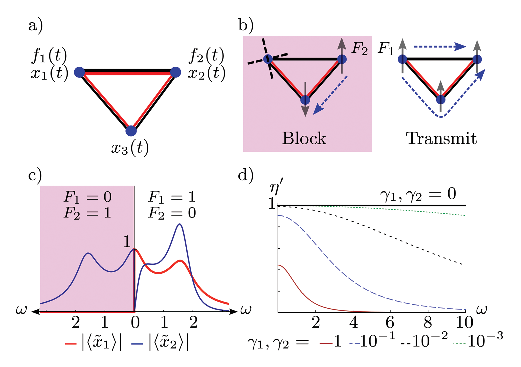
\includegraphics{epl17030f1_pr.eps}
\caption{(Colour on-line) (a) Three-oscillator system with variables $x_{1,2,3}$ where oscillators~1 and~2 can be forced. Red and black lines symbolize coupling with $b$, $\kappa$, respectively. (b)~Working principle of the three-oscillator diode. (c) Exemplary diode response from a solution of eqs.~(\ref{epl17030eqn2}),~(\ref{epl17030eqn3}) with parameter conditions for example 1 and $\gamma_1=0.2$, $\gamma_2=0.1$. Left:~blocking state; right:~transmitting state. (d)~Efficiency at maximum power $\eta'$ of the diode approaches unity when $\gamma_1$ and $\gamma_2$ vanish. Parameters:~$\kappa_{11}=\kappa_{22}=2$, $\kappa_{13}=\kappa_{23}=-1$, $b_{23}=1$, $\gamma_3 =2$.}
\label{epl17030fig1}
\vspace*{-10pt}
\end{figure}

For broken Onsager symmetry, the direction of the energy flow and hence the choice of input and output oscillators generally matters. In the following, the index $b$ will be used for the oscillator that provides energy output. Then, the efficiency of the energy transfer can be defined~as
\begin{equation}%eq8
\eta \equiv -\dot{W}_b/\dot{W}_a = -\dot{W}_b/(-\dot{W}_b + \dot{W}_{\text{diss}}) \leq 1.
\label{epl17030eqn8}
\end{equation}
A key figure of merit is the efficiency at maximum power output, which is here defined for fixed frequencies as
\begin{equation}%eq9
\eta^{\prime} \equiv \eta(-\dot{W}_b |_{{\omega}} \rightarrow \max),
\label{epl17030eqn9}
\end{equation}
where the maximum $-\dot{W}_b |_{{\omega}} $ of the power output is found by searching for an optimal phase difference $\varphi_{ba}$ and \nobreak{magnitude} of the driving force $f_b$. In linear systems with conserved Onsager symmetry efficiency at maximum power is generally expected to be smaller than $1/2$~\cite{epl17030bib16}. However, the following examples will demonstrate that networks of the type of eq.~(\ref{epl17030eqn1}) do not necessarily obey such an energetic constraint. Moreover, the interplay of network topology and local breaking of Onsager symmetry will \nobreak{allow} further truly remarkable properties.

\section{Example 1: a highly efficient diode}

Consider a network of three oscillators as depicted in fig.~\ref{epl17030fig1}(a). The dynamics is described by eq.~(\ref{epl17030eqn1}) where $j=1\ldots3$, thus we have
\begin{small}
\begin{eqnarray*}
\mathbf{A}=\begin{pmatrix}
\kappa_{11}-\omega^2+i\omega\gamma_1 &\kappa_{12}+i\omega b_{12} &\kappa_{13}+i\omega b_{13} \\[1pt]
\kappa_{12}-i\omega b_{12} & \kappa_{22}-\omega^2+i\omega\gamma_2& \kappa_{23}+i\omega b_{23}\\[1pt]
\kappa_{13}-i\omega b_{13} & \kappa_{23}-i\omega b_{23} & \kappa_{33}-\omega^2+i\omega\gamma_3
\end{pmatrix},
\end{eqnarray*}
\end{small}%
which yields a lengthy expression for $\bm{\chi}$ on inversion. Broken Onsager symmetry now allows to choose coupling \nobreak{parameters} in $\mathbf{A}$ such as to have $\chi_{12}(\omega)=0$ for any frequency while $\chi_{21}(\omega)\neq0$. This condition yields the parameters $b_{12} = 0,\; b_{13} = -\kappa_{12}/b_{23},\; \kappa_{33} = \kappa_{13} \kappa_{23}/\kappa_{12}$, and $\kappa_{12} = -(\kappa_{13} b_{23}^2)/(\kappa_{23} + b_{23} \gamma_3)$. Note that stability conditions on $\bm{\kappa}$ now impose a stronger constraint on the remaining free parameters. As illustrated in fig.~\ref{epl17030fig1}(b), (c) the system is a dynamic, but genuine diode. Forcing with $f_2$ always leads to an anti-phase effect of oscillators~2 and~3 on oscillator 1, which completely blocks the response of the latter. In contrast, forcing with $f_1$ leads to no cancellation of 1 and 3, such that the energy can be carried around both sides of the structure.

\looseness-1In fig.~\ref{epl17030fig1}(d) the efficiency at maximum power $\eta'$ is displayed. Explicit expressions can be found in the following sections. For this diode $\eta'$ generally has only one maximum located at $\omega=0$. As shown, the system can asymptotically reach a unit efficiency at maximum power, which is achieved when friction in oscillators $1$ and $2$ vanish since $\lim_{(\gamma_1,\gamma_2) \rightarrow 0}\eta' = 1$. In contrast to systems with conserved Onsager symmetry, this diode can reach its upper bound of efficiency at almost arbitrary values of $\gamma_3$. Analytical calculations for $\gamma_3 \rightarrow \infty$ show that the upper bound of $\eta'$ is reached when $\gamma_{1,2}$ tend to zero as $\gamma_3^{-h}$ with $h>1$. In the limit $\gamma_3 \rightarrow 0$, the system always becomes unstable since $\bm{\kappa}$ is then no longer positive definite. It should be emphasized that the theoretical reachability of $\eta'\approx 1$ in a genuine linear-response steady state makes this new diode unique.

\section{Example 2: isolated transmission chain}

The working principle of the diode in example~1 can also \nobreak{allow} for isolation of energy transfer in spatially extended systems. Consider two chains as shown in fig.~\ref{epl17030fig2}(a), consisting of $N+1$ and $N-1$ oscillators, respectively. The sought-for isolation mechanism should allow energy transfer in the lower chain without exciting the upper chain. The oscillating variables of upper and lower chains $x^{\text{u}}_{j}$, $x^{\text{l}}_{j}$ are assumed to obey
\begin{eqnarray}%eq10
\ddot{x}^{\text{u}}_{j}&=&\kappa \left[x^{\text{u}}_{j-1}+x^{\text{u}}_{j+1}-2 x^{\text{u}}_{j} \right] + d \left[x^{\text{l}}_{j}-x^{\text{u}}_{j}\right] -\gamma_{\text{u}} \dot{x}^{\text{u}}_j\nonumber\\
&& +\, b\left[\dot{x}^{\text{l}}_{j-1}+\dot{x}^{\text{l}}_{j+1}\right],\nonumber\\
\ddot{x}^{\text{l}}_{j}&=&\kappa\left[x^{\text{l}}_{j-1}+x^{\text{l}}_{j+1}-2 x^{\text{l}}_{j}\right] + d \left[x^{\text{u}}_{j}-x^{\text{l}}_{j}\right]-\gamma_{\text{l}}\dot{x}^{\text{l}}_{j}\nonumber\\
&&-\, b\left[\dot{x}^{\text{u}}_{j-1}+\dot{x}^{\text{u}}_{j+1}\right],\label{epl17030eqn10}
\end{eqnarray}
where noise is dropped for simplicity and the constants of time-reversal symmetric couplings are denoted by $\kappa, d$. The boundary conditions at the ends of the chains are given below\footnote{The boundary conditions for the chains in example 2 read
\begin{eqnarray*}
\ddot{x}^{\text{l}}_0&=&\kappa [x^{\text{l}}_1- x^{\text{l}}_0] -\gamma_{\text{l}} \dot{x}^{\text{l}}_0 - b \dot{x}^{\text{u}}_1 + f_0,\\[2.5pt]
\ddot{x}^{\text{l}}_N &=&\kappa [x^{\text{l}}_{N-1}- x^{\text{l}}_N] -\gamma_{\text{l}} \dot{x}^{\text{l}}_N - b \dot{x}^{\text{u}}_{N-1} + f_N,\\[2.5pt]
\ddot{x}^{\text{u}}_1 &=&\kappa [x^{\text{u}}_2- x^{\text{u}}_1] + d [x^{\text{l}}_1-x^{\text{u}}_1] -\gamma_{\text{u}} \dot{x}^{\text{u}}_1 +b [\dot{x}^{\text{l}}_0+\dot{x}^{\text{l}}_2],\\[2.5pt]
\ddot{x}^{\text{u}}_{N-1} &=&\kappa [x^{\text{u}}_{N-2}- x^{\text{u}}_{N-1}] + d [x^{\text{l}}_{N-1}-x^{\text{u}}_{N-1}] -\gamma_{\text{u}} \dot{x}^{\text{u}}_{N-1}\\[2.5pt]
&&+\,b [\dot{x}^{\text{l}}_{N}+\dot{x}^{\text{l}}_{N-2}]\\[-1.7pc]
\end{eqnarray*}}. Isolated energy transfer requires a cancellation mechanism in the upper chain that holds for both forward- and backward-traveling waves.~Therefore, the system is made left-right symmetric by giving the two magnetic couplings with $b$ at each oscillator in eq.~(\ref{epl17030eqn10}) always the same sign. The wave mode ansatz $(\tilde{x}^{\text{u}}_{\alpha},\tilde{x}^{\text{l}}_{\alpha})\,e^{i(\omega t - k_{\alpha}\,j)}$ in eq.~(\ref{epl17030eqn10}) yields
\begin{small}
\begin{eqnarray}%eq11
&&\begin{pmatrix}
w^2-2\kappa(1-\cos(k_{\alpha}))-d-i\omega \gamma_{\text{u}}\ d+i\omega 2b\cos(k_{\alpha})\\[4pt]
d-i\omega 2b \cos(k_{\alpha})\ w^2-2\kappa(1-\cos(k_{\alpha}))-d-i\omega \gamma_{\text{l}}
\end{pmatrix}\begin{pmatrix}
\tilde{x}^{\text{u}}_{\alpha}\\[4pt]
\tilde{x}^{\text{l}}_{\alpha}
\end{pmatrix}\nonumber\\
&&=\,0.
\label{epl17030eqn11}
\end{eqnarray}
\end{small}%
The asymmetry of the matrix in eq.~(\ref{epl17030eqn11}) allows $\tilde{x}^{\text{u}}$ to be independent of $\tilde{x}^{\text{l}}$ if the upper off-diagonal and the lower diagonal entries vanish. Such a state can be achieved if the parameters are chosen as $b = \kappa/\sqrt{d + 2\kappa}$, $\gamma_{l} = d/\sqrt{d + 2\kappa}$ and the forcing frequency is $\omega_I\equiv\sqrt{d + 2\kappa}$. Equation~(\ref{epl17030eqn11}) then yields the wave vectors $k_{1,2} =\pm\arccos(i\,d/(2\kappa))+2\pi\,n$, $n\in \mathbb{Z}$. Given proper boundary conditions$^{2}$, we now have a one-way isolation of the upper chain from the lower chain as illustrated by the responses $x_j^{\{\text{u},\text{l}\}}$ in fig.~\ref{epl17030fig2}(b). Note that isolation is here independent of the phase between the forces $\varphi_{0 N}$ and force magnitudes $F_{\{0,N\}}$.~Energy transmission is now also insensitive to spatial variations or friction in the upper chain.

\begin{figure}[t]%fig2
\centering
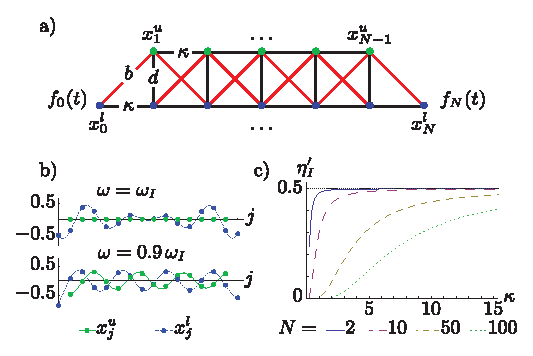
\includegraphics{epl17030f2_pr.eps}
\caption{(Colour on-line) (a)~Oscillator system that allows mono-directional isolation of the upper chain from the lower chain. (b)~Snapshots of the whole-chain responses $x_{j}^{\{\text{u},\text{l}\}}(t)$ for ${t=0} \ (N=15)$. Top graph: when driven at the frequency $\omega_I$, the upper chain is not excited by the energy transfer in the isolated lower chain. Bottom graph: driving at any other frequency leads to excitations in both chains. (c)~Efficiency at maximum power for isolated energy transfer through the lower chain at $\omega_I$. Here, time reversibility of couplings is conserved in the isolated state, thus $\eta_I^{\prime}\leq1/2$. Parameters:~$F_0=1$, $d=0.1$, $\gamma_{\text{u}}=0.1$.}
\label{epl17030fig2}
\vspace*{-10pt}
\end{figure}

\section{General rules for mono-directional transport}

Diode-like directional links as in example 1 can emerge in any network with broken Onsager symmetry when off-diagonal elements of the complex admittance vanish asymmetrically. If excitations are to travel from oscillator $j$ to $l$ but not the reverse way, the following conditions must hold for any $\omega$:
\begin{equation}%eq12
\chi_{jl} = (-1)^{i+j}\frac{\mathrm{det}\left(\mathbf{A}_{(lj)}\right)}{\mathrm{det}\left(\mathbf{A}\right)} = 0, \quad \chi_{lj} \neq 0.
\label{epl17030eqn12}
\end{equation}
Here, $\chi_{jl}=(\mathbf{A})^{-1}_{jl}$ is expressed with the submatrix $\mathbf{A}_{(lj)}$ that results on elimination of row $l$ and column $j$ from $\mathbf{A}$. To design a network with mono-directional links, system parameters must be determined by solving an expansion of eq.~(\ref{epl17030eqn12}) for all orders of $\omega$, which can be tedious. However, inspection of the network topology already provides important insight about the feasibility of such links in systems of type~(\ref{epl17030eqn1}). Three general rules are found to hold, and are illustrated in fig.~\ref{epl17030fig3}:

\begin{enumerate}

\item[1)] Mono-directional links require network loops.
\item[2)] A mono-directional link between immediately coupled oscillators requires a loop of three oscillators.
\item[3)] No oscillator can be connected in a totally mono-directional way where all links are directed towards or away from it.
\end{enumerate}
Brief derivations are given in the last section of this \nobreak{letter}. Rule~1) can be understood intuitively by \nobreak{thinking} of mono-directional transport as intrinsic negative interference that occurs only in one direction. Since interference requires superposition of at least two signals, the necessity of loops is plausible. An extension of this argument provides physical understanding of the second rule. Rule~2) derives from matching of powers of $\omega$ for the high-frequency limit of eq.~(\ref{epl17030eqn12}). Here, a direct connection between two oscillators picks up the same power of $\omega$ as an indirect, magnetic coupling via a third oscillator. In order to balance each other, both must be present. Note that rule~2) also holds when different oscillators in the system~(\ref{epl17030eqn1}) are augmented with individual, but non-zero, ``mass'' factors at the second time derivatives.

Rule~3) can be justified by an interesting thermodynamical interpretation: Consider for now a force-free situation $f_j=0$ and assume that the oscillators are embedded in individual heat baths, keeping them at different temperatures. The resulting variation of noise levels leads to preferred dissipation at the ``colder'' oscillators. Heat exchange is given by the deviations of the kinetic oscillator temperatures from the temperatures $T_j$ of the heat baths as $\dot{Q}_j = \gamma_j(\langle \dot{x}_j^2\rangle - k_{\text{B}}\,T_j)$~\cite{epl17030bib17}. If it was now possible to connect one oscillator $j$ in a totally mono-directional way to all the rest of the network, heat would always flow either towards $j$ or away from $j$, regardless of the temperature difference. Such a network is physically impossible since it would allow the construction of a perpetuum mobile and violate the second law of thermodynamics.

\begin{figure}[t]%fig3
\centering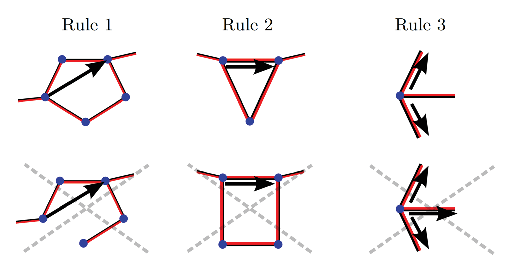
\includegraphics{epl17030f3_pr.eps}
\caption{(Colour on-line) Illustration of the rules that constrain mono-directional transport in arbitrary networks. Black arrows are mono-directional links where excitations can only travel in one direction. Red/black lines indicate any coupling $(b_{jl},\ \kappa_{jl})$.}
\label{epl17030fig3}
\vspace*{-12pt}
\end{figure}

\section{Topology and efficiency at maximum power}

To substantiate the conclusions drawn from example 1 above, this section provides general formulae and limits for the efficiency at maximum power. We begin by rewriting the work rates conveniently in Fourier space with the complex admittance split into real $\Re(\chi_{jl})$ and imaginary $\Im(\chi_{jl})$ parts. Using $j,l\in\{a,b\}$ for the input and output, we have from eq.~(\ref{epl17030eqn6})
\begin{eqnarray}%eq13,14
\dot{W}_j &=&i \omega \sum_l\left(\tilde{f}^{*}_j\chi_{jl}\tilde{f}_l - \tilde{f}^{ }_j\chi^{*}_{jl}\tilde{f}^{*}_l\right)
\label{epl17030eqn13}\\
&=& -2\omega|\tilde{f}_j|^2 \Im(\chi_{jj})-2\omega \sum_{l\neq j} |\tilde{f}_j||\tilde{f}_l| \alpha_{jl},
\label{epl17030eqn14}
\end{eqnarray}
where $\alpha_{jl}$ is a function of the phase difference $\varphi_{jl}$ as
\begin{equation}%eq15
\alpha_{jl} \equiv \Im(\chi_{jl})\cos(\varphi_{jl})-\Re(\chi_{jl})\sin(\varphi_{jl}).
\label{epl17030eqn15}
\end{equation}
Inserting eq.~(\ref{epl17030eqn13}) into the formula for overall dissipation~(\ref{epl17030eqn7}), the condition $\dot{W}_{\text{diss}} \geq 0$
requires positive semi-definiteness of the matrix $i(\chi_{jl}-\chi_{lj}^{*})$.

To calculate efficiency at maximum power $\eta'$, we first maximize $\dot{W}_b$ with respect to phase and force. Variables with values at maximum power are primed $(')$. On setting the $\varphi_{ba}$ and $|\tilde{f}_b|$ derivatives of $\dot{W}_b$ in eq.~(\ref{epl17030eqn14}) equal to zero we find $\tan{\varphi'_{ba}} = -\Re{(\chi_{ba})}/\Im{(\chi_{ba})}$ and $|\tilde{f}'_a|/|\tilde{f}'_b| = -2 \Im{(\chi_{bb})}/{\alpha'_{ba}}$ with ${\alpha'}^{2}_{ba}=\alpha_{ba}(\varphi_{ba}')^2 = |\chi_{ba}|^2$. Some care must be taken when selecting $\varphi'_{ba}$ since work is periodic in the phase. The maximum power output becomes
\begin{equation}%eq16
\dot{W}_b^{\prime} = \omega\,{\alpha'}^2_{ba}\,|\tilde{f}'_a|^2/(2\,\Im{(\chi_{bb})}).
\label{epl17030eqn16}
\end{equation}
The above relations can be straightforwardly inserted into eqs.~(\ref{epl17030eqn8}),~(\ref{epl17030eqn14}) to obtain for the efficiency at maximum power
\begin{align}%eq17
\eta' = \frac{{\alpha'}^2_{ba}}{2 \left( 2\Im(\chi_{bb})\Im(\chi_{aa}) - \alpha'_{ba} \alpha'_{ab}\right)} \leq 1.
\label{epl17030eqn17}
\end{align}
As demonstrated in fig.~\ref{epl17030fig1} for example 1, the bound $\eta'=1$ can indeed be reached asymptotically when Lorentz-force--like couplings are present. Note, however, that this high efficiency $\eta'$ does not require in general mono-directional links.

Next, we calculate the efficiency at maxium power when Onsager symmetry holds. Thus, we set $\mathbf{b}=\mathbf{0}$. Using the symmetry of $\bm{\chi}$ together with the above conditions determining $\varphi'_{ba}$ and $\alpha'_{ba}$ we have here ${\alpha'}_{ab}^{2} = -{\alpha'}_{ba}^{2}(\cos^2(\varphi_{ba}')-\sin^2(\varphi'_{ba}))^2$. The efficiency at maximum power for networks with Onsager symmetry results in
\begin{equation}%eq18
\eta'_{s} = \frac{1}{2\left([\frac{2\Im(\chi_{bb})\Im(\chi_{aa})}{\Im(\chi_{ba})^2}-1]\cos^2(\varphi'_{ba}) + \sin^2(\varphi'_{ba})\right)} \leq \frac{1}{2}.
\label{epl17030eqn18}
\end{equation}
The last inequality follows from $\Im(\chi_{bb})\Im(\chi_{aa})\geq\Im(\chi_{ab})^2$, which is for symmetric $\bm{\chi}$ equivalent to $\dot{W}_{\text{diss}} \geq 0$. The here-derived bound of $1/2$ is analogous to the Curzon-Ahlborn limit for heat machines~\cite{epl17030bib16,epl17030bib18,epl17030bib19}. In the quasistatic limit of vanishing $\omega$ we have $0\approx\Im{(\chi_{ba})} \approx \Im{(\chi_{bb})}$. Therefore, $\cos{\varphi'_{ba}} \approx 0$ and $|\tilde{f}'_a|/|\tilde{f}'_b| \approx 0$. Consequently, for conserved Onsager symmetry, the efficiency at maximum power attains its absolute maximum at vanishing driving frequency $\lim_{\omega\rightarrow 0}\eta' = 1/2$ and the transmitted power vanishes here. On the other hand, it is possible to show with examples that the absolute maximum of $\eta'$ need not be located at $\omega=0$ when Lorentz-force--like couplings are present.

Finally, we investigate the case of broken Onsager symmetry for a network without loops. In such a system each connected pair of elements is connected via a unique path, which allows to express $\bm{\chi}$ as follows~\cite{epl17030bib20}. Consider a path from oscillator with index $j$ to oscillator $l$ and denote the overall number of oscillators on the path by $n_p$. Since the sequence of indices on the path may be non-monotonic, we rename them by $k_1\ldots k_{n_p}$ where $k_1=j$ and $k_{n_p}=l$. For $j\neq l$ the inverse of the non-singular matrix $\mathbf{A}$ can then be written as
\begin{equation}%eq19
\chi_{jl} = \left[\frac{(-1)^{n_p-1}\mathrm{det}(\mathbf{A}_{(j-l)})}{\mathrm{det}(\mathbf{A})}\right]\left[\prod^{n_p -1}_{m=1} A_{k_m,k_{m+1}}\right] \equiv C\,K,
\label{epl17030eqn19}
\end{equation}
where $\mathbf{A}_{(j-l)}$ denotes the submatrix from which all the rows and columns carrying indices corresponding to elements of the path are removed. When $n_p = 2$ we \nobreak{replace} $\det(\textbf{A}_{(j-1)})$ by unity. Only the factor $K$, representing the second bracket, depends on the direction of the path. For our systems~(\ref{epl17030eqn1}), we have $A_{k_m,k_{m+1}}=A_{k_{m+1},k_{m}}^{*}$ and the reverse path thus yields $\chi_{lj} = C\,K^{*}$. This relation is now used together with the maximum-power condition for $\varphi'_{ba}$ in eq.~(\ref{epl17030eqn15}) to give $(\alpha'_{ba})^2 = |CK|^2$ and $\alpha'_{ab}\alpha'_{ab} = -[C^2+(C^*)^2]|K|^2/2$. Inserting everything in eq.~(\ref{epl17030eqn17}) yields for any loop-free system
\begin{equation}%eq20
\eta'_{l} = \frac{1}{2 + 4\left(\Im(\chi_{bb})\Im(\chi_{aa}) - |K|^2 \Im(C)^2\right)/(|C|^2 |K|^2)} \leq \frac{1}{2},
\label{epl17030eqn20}
\end{equation}
where the bound follows from positivity of energy dissipation, eqs.~(\ref{epl17030eqn7}),~(\ref{epl17030eqn14}).~This equation shows that achieving an efficiency at maximum power larger than $1/2$ not only requires broken Onsager symmetry, but also network loops.

\section{Tunable high-frequency efficiency}

A further energetic advantage of Lorentz-force--like coupling occurs when a direct link $b_{ab}\neq 0$ between input and output exists. An expansion of efficiency, eq.~(\ref{epl17030eqn8}) with eq.~(\ref{epl17030eqn14}), shows that systems of type~(\ref{epl17030eqn1}) all have the same high-frequency limit
\begin{equation}%eq21
\lim\limits_{\omega \rightarrow \infty} \eta = \max\left(\frac{-|\tilde{f}_b|^2 \gamma_b + |\tilde{f}_a| |\tilde{f}_b| b_{ab} \cos{\varphi_{ab}}}{|\tilde{f}_a|^2 \gamma_a + |\tilde{f}_a||\tilde{f}_b| b_{ab} \cos{\varphi_{ab}}},0\right).
\label{epl17030eqn21}
\end{equation}
Lorentz-force--like coupling thus allows to extend the good \nobreak{efficiency} to high frequencies.

\section{Fluctuations and multiplicative noise}

The network equation~(\ref{epl17030eqn1}) contains a source of additive noise $\xi_j$ for completeness. Such noise does not affect the results in this article. Mechanisms for mono-directional transport depend only on system parameters and apply to noise-driven excitations as much as to any other excitation. In contrast to other definitions of efficiency~\cite{epl17030bib21}, the here-defined efficiency $\eta$ does not fluctuate. Concerning the work rates, eq.~(\ref{epl17030eqn6}), these contain expectation values $\langle x_j\rangle$ and additive noise is thus averaged out.

However, multiplicative noise resulting from parameter fluctuations, in particular from unsteady magnetic fields, could have a more pronounced effect.~On using the~Stratonowich interpretation it can be shown that white noise in $\mathbf{b}$ renormalizes the friction constants $\gamma_j$ in the~equation for the first moments of $x_j$~\cite{epl17030bib22}. Multiplicative noise in $\mathbf{b}$ increases the effective friction, but does not lead to instabilities. Therefore, the principles described in this letter continue to work for averages when the magnetic coupling fluctuates. Mono-directional transport \nobreak{remains} possible on average.

\section{Concluding perspectives}

Although linear oscillators are an established paradigm of physics, the \nobreak{energetics} of oscillator networks with Lorentz-force--like couplings has hardly been explored. Focussing on networks with only the most generic types of coupling, it has been shown here that unusual transport properties entail favorable energetics and result from the interplay of network topology and time-reversal symmetry breaking.

Other types of couplings could also be studied with the present framework. Firstly, one could consider frictional/resistive interaction of the network elements via a symmetric matrix of coefficients $\gamma_{jl}$. With such coupling the off-diagonal elements of $\mathbf{A}$ no longer form a Hermitian matrix and the above rules do not hold. Most notably, a diode-like device could be made in a system with only two elements. Combining here a magnetic coupling $b_{12}$ with an equally strong frictional/resistive force $\gamma_{12}=b_{12}$ yields a diode since the off-diagonal elements become $A_{21}=-i \omega b_{12}+i \omega \gamma_{12}=0$ and $A_{12}=2 i \omega \gamma_{12}$, respectively. Such a device has been realized using a Hall element~\cite{epl17030bib23,epl17030bib11}. However, frictional coupling causes extra dissipation and one might therefore expect that this article's mechanisms for mono-directional transport generally display a superior efficiency. Secondly, one could generalize the system through coupling of the second time derivatives. Such coupling is realized physically by shared moments of inertia or by mutual induction. It affects the high-$\omega$ regime and allows efficient energy transfer there. Finally, one could go beyond the assumption of network linearity. In this case, the efficiency at maximum power is generally not limited by $1/2$, even when Onsager symmetry is conserved~\cite{epl17030bib18}. Besides energetic issues, it might also be interesting to study correlations or synchronization~\cite{epl17030bib26,epl17030bib24,epl17030bib25} of non-linear oscillators in networks with Lorentz-force--like couplings.

It is tempting to speculate about a few applications of the studied system. Periodic structures related to the oscillator chain in example~2 might allow for \hbox{cloaking-inspired}~\cite{epl17030bib27} mono-directional shielding.~Mechanical devices, such as a mono-directional vibration damper, are at least in principle conceivable. Realization of the suggested high efficiency in electric circuits hinges on the availability of low-resistance symmetry-breaking couplings~\cite{epl17030bib28,epl17030bib29,epl17030bib30}. With these, efficient magnetic-field programmable networks could operate much like a transistor circuit, with the major distinction of being linear.

\acknowledgments{The author is indebted to Prof.~\textsc{U.~Seifert} for long-standing support and for discussions. Prof.~\textsc{H.~A.~Stone} is thanked for comments on the manuscript. A postdoctoral fellowship from the DAAD is acknowledged.}

\section{Appendix: brief derivations of rules 1--3}

\textit{Rule~1: Mono-directional links require network loops}. This rule is shown most easily with eq.~(\ref{epl17030eqn19}) by \nobreak{demonstrating} that conditions~(\ref{epl17030eqn12}) cannot be satisfied in a connected, but acyclic system. Since the offdiagonal elements of $\mathbf{A}$ are Hermitian, $\chi_{lj}$ and $\chi_{jl}$ are here related to each other through complex conjugation of the terms $\sim A_{k_m,k_{m+1}}$ in the factor $K$. Thus, if $\chi_{jl}=C\,K=0$, also $\chi_{lj}= C K^{*}=0$ and diode-like behavior is impossible.

\textit{Rule~2: A mono-directional link between immediately coupled oscillators requires a loop of three oscillators}. This rule demands a direct link between $j$ and $l$, therefore we assume $a_{jl}+i\omega b_{jl} \neq 0$. On using the Leibniz formula for determinants it can be shown that
\begin{eqnarray*}
\chi_{jl} &\sim& \mathrm{det}\left(\mathbf{A}_{(lj)}\right) = i b_{jl}\omega^{2N_o-3} + b_{jl} \sum_{m,m\notin\{j,l\}}\gamma_m \omega^{2N_o-4}\\
&&+\,\left[\kappa_{jl}-\sum_{m,m\notin\{j,l\}}b_{ml}b_{jm}\right] \omega^{2N_o-4} + O(\omega^{2N_o-5}),\label{eq_rule2_expansion}
\end{eqnarray*}
where $N_o$ is the number of oscillators in the system. This expansion is to vanish for all $\omega$. Hence, the first term requires $b_{jl}=0$. In the bracketed expression, $\kappa_{jl}$ can only be balanced by a non-zero last term $\sim b_{ml}b_{jm}$. This last term requires oscillators with index $m$ that are directly connected to both oscillators $j$ and $l$, hence making a loop of three oscillators necessary.

\textit{Rule~3: No oscillator can be connected in a totally mono-directional way}. Assuming that an oscillator with index $k$ has only mono-directional links, we show that such a system would have unphysical properties. According to eq.~(\ref{epl17030eqn12}), we require for all $j$ with $j\neq k$ that $\chi_{kj} \sim \mathrm{det}\left(\mathbf{A}_{(jk)}\right) = 0$. On using this statement in Laplace's formula the determinant of the system matrix becomes
\begin{equation*}
\mathrm{det}\left(\mathbf{A}\right) = \sum_{j} A_{jk} (-1)^{k+j}\mathrm{det}\left(\mathbf{A}_{(jk)}\right) = A_{kk} \det\left(\mathbf{A}_{(kk)}\right).
\end{equation*}
However, on writing out $\mathrm{det}\left(\mathbf{A}_{(jk)}\right) = 0$ for all $j$'s with $j\neq k$ it becomes clear that also $\mathrm{det}\left(\mathbf{A}_{(kk)}\right)=0$ since\vadjust{\vspace*{-4pt}\pagebreak} all rows in $\mathbf{A}_{(kk)}$ are made linearly dependent on each other if $A_{kj, j\neq k}\neq 0$. Therefore, we have $\mathrm{det}\left(\mathbf{A}\right)=0$ and a totally mono-directional coupling of $k$ would make the system singular, which is unphysical.

\begin{thebibliography}{99}

\bibitem{epl17030bib1}
\Name{Benenti G., Saito K. \and Casati G.}
\REVIEW{Phys. Rev. Lett.}{106}{2011}{230602}.

\bibitem{epl17030bib2}
\Name{B{\"u}ttiker M., Imry Y., Landauer R. \and Pinhas S.}
\REVIEW{Phys. Rev. B}{31}{1985}{6207}.%\vadjust{\vspace*{0.83pc}\pagebreak}

\bibitem{epl17030bib3}
\Name{Brandner K., Saito K. \and Seifert U.}
\REVIEW{Phys. Rev. Lett.}{110}{2013}{070603}.

\bibitem{epl17030bib4}
\Name{Whitney R.~S.}
\REVIEW{Phys. Rev. Lett.}{112}{2014}{130601}.

\bibitem{epl17030bib5}
\Name{Brandner K. \and Seifert U.}
\REVIEW{Phys. Rev. E}{91}{2015}{012121}.

\bibitem{epl17030bib6}
\Name{Allahverdyan A.~E., Hovhannisyan K.~V., Melkikh A.~V. \and Gevorkian
 S.~G.}
 \REVIEW{Phys. Rev. Lett.}{111}{2013}{050601}.

\bibitem{epl17030bib7}
\Name{Stark J., Brandner K., Saito K. \and Seifert U.}
\REVIEW{Phys. Rev. Lett.}{112}{2014}{140601}.

\bibitem{epl17030bib8}
\Name{Carmi S., Wu Z., Havlin S. \and Stanley H.~E.}
\REVIEW{EPL}{84}{2008}{28005}.

\bibitem{epl17030bib9}
\Name{Rohden M., Sorge A., Timme M. \and Witthaut D.}
\REVIEW{Phys. Rev. Lett.}{109}{2012}{064101}.

\bibitem{epl17030bib10}
\Name{Tellegen B.~D.}
\REVIEW{Philips Res. Rep.}{3}{1948}{81}.

\bibitem{epl17030bib11}
\Name{Wick R.~F.}
\REVIEW{J. Appl. Phys.}{25}{1954}{741}.

\bibitem{epl17030bib12}
\Name{Grubbs W.}
\REVIEW{Bell Syst. Tech. J.}{38}{1959}{853}.

\bibitem{epl17030bib13}
\Name{Hogan C.~L.}
\REVIEW{Rev. Mod. Phys.}{25}{1953}{253}.

\bibitem{epl17030bib14}
\Name{Strogatz S.~H.}
\Book{Nonlinear Dynamics and Chaos}
\Publ{Perseus Publishing}
\Year{1994}.

\bibitem{epl17030bib15}
\Name{Hashitsume N., Toda M., Kubo R. \and Sait{\=o} N.}
\Book{\nobreak{Statistical} Physics II}
\Publ{Springer}
\Year{1992}.

\bibitem{epl17030bib16}
\Name{Curzon F. \and Ahlborn B.}
\REVIEW{Am. J. Phys.}{43}{1975}{22}.

\bibitem{epl17030bib17}
\Name{Sekimoto K.}
\REVIEW{Progr. Theor. Phys. Suppl.}{130}{1998}{17}.

\bibitem{epl17030bib18}
\Name{Esposito M., Lindenberg K. \and Van~den Broeck C.}
\REVIEW{Phys. Rev. Lett.}{102}{2009}{130602}.

\bibitem{epl17030bib19}
\Name{Van~den Broeck C., Kumar N. \and Lindenberg K.}
\REVIEW{Phys. Rev. Lett.}{108}{2012}{210602}.

\bibitem{epl17030bib20}
\Name{Klein D.}
\REVIEW{Linear Algebra Appl.}{42}{1982}{109}.

\bibitem{epl17030bib21}
\Name{Verley G., Esposito M., Willaert T. \and Van~den Broeck C.}
\REVIEW{Nat. Commun.}{5}{2014}{4721}.

\bibitem{epl17030bib22}
\Name{Sabass B.} in preparation.

\bibitem{epl17030bib23}
\Name{Mason W., Hewitt W. \and Wick R.}
\REVIEW{J. Appl. Phys.}{24}{1953}{166}.

\bibitem{epl17030bib24}
\Name{J{\"u}licher F., Dierkes K., Lindner B., Prost J. \and Martin P.}
 \REVIEW{Eur. Phys. J. E}{29}{2009}{449}.

\bibitem{epl17030bib25}
\Name{Ren J., Wang W.-X., Li B. \and Lai Y.-C.}
\REVIEW{Phys. Rev. Lett.}{104}{2010}{058701}.

\bibitem{epl17030bib26}
\Name{Martens E.~A., Thutupalli S., Fourri{\`e}re A. \and Hallatschek O.}
\REVIEW{Proc. Natl. Acad. Sci. U.S.A.}{110}{2013}{10563}.

\bibitem{epl17030bib27}
\Name{Pendry J.~B., Schurig D. \and Smith D.~R.}
\REVIEW{Science}{312}{2006}{1780}.

\bibitem{epl17030bib28}
\Name{Zhai J., Li J., Dong S., Viehland D. \and Bichurin M.}
\REVIEW{J. Appl. Phys.}{100}{2006}{124509}.

\bibitem{epl17030bib29}
\Name{Viola G. \and DiVincenzo D.~P.}
\REVIEW{Phys. Rev. X}{4}{2014}{021019}.

\bibitem{epl17030bib30}
\Name{Estep N.~A., Sounas D.~L., Soric J. \and Al{\`u} A.}
\REVIEW{Nat. Phys.}{10}{2014}{923}.

\end{thebibliography}

\end{document}


